\documentclass[a4paper, 11pt]{article}

% -- Coments
\usepackage{verbatim}

\usepackage{array}
\usepackage{makecell}
\usepackage{tikz}

% ----- Fonts -----
% -- Fuente --
% \usepackage{fontspec}
% \setmonofont{JetBrainsMono Nerd Font}  

% -- Color --
\usepackage{xcolor}
%\definecolor{azul}{RGB}{00,33,99}
\definecolor{azul}{RGB}{35,72,180}

% -- Page Margin --
\usepackage[margin=1in]{geometry}

% -- Espaciados --
\newcommand{\Pspace}{0.5cm}
\newcommand{\Aspace}{0.2cm}
\setlength{\parindent}{0pt}

% -- Columnas --
\usepackage{multicol}

% -- Imagenes --
\usepackage{graphicx}
\usepackage{float}

% -- Matemáticas --
\usepackage{amsmath, amssymb}

% -- Gráficas --
\usepackage{pgfplots}
\pgfplotsset{compat=1.18}

% -- Código --
\usepackage{listings}
\lstset{
    language=C++,                   % Lenguaje del código
    basicstyle=\ttfamily\small,     % Fuente del código
    keywordstyle=\color{blue},      % Color de palabras clave
    commentstyle=\color{gray},      % Color de comentarios
    stringstyle=\color{red},        % Color de cadenas
    numbers=left,                   % Números de línea a la izquierda
    numberstyle=\tiny\color{gray},
    breaklines=true,                % Permitir saltos de línea
    frame=single                    % Marco alrededor del código
}

\begin{comment}
-- Formato de pregunta simple
    % - Problema n
    \vspace{\Pspace}
    \item Problema \par
        % Respuesta:
        \vspace{\Aspace} \par
        { \color{azul}  }


 -- Formato de pregunta multimple
        % - Problema 
        \vspace{\Pspace}
        \item  \par
             % Respuestas:
            \vspace{\Aspace} \par
            a) 
            \\ { \color{azul} }

            \vspace{\Aspace} \par
            b) 
            \\ { \color{azul} }


 -- Formato de imagen
\begin{figure}[!ht]
    \centering
    \includegraphics[width=0.5\textwidth]{}
\end{figure}


 -- Formato de tabla
\begin{tabular}{c|c}
    \textbf{A} & \textbf{B} \\
    \hline
    Texto & Texto \\
    Texto & Texto
\end{tabular} \\
\end{comment}


\title
{
    Sistemas Operativos 2026-2 \\
    Unidad II - Tareas y Procesos
}

\begin{document}

\maketitle

\begin{center}
    \begin{tabular}{r|l}
        \textbf{Expediente} & \textbf{Nombre} \\ \hline
        219208106 & Bórquez Guerrero Angel Fernando \\
    \end{tabular}
\end{center}

\rule{\linewidth}{0.3mm}

\vspace{0.3cm}
\section{Concepto de proceso}
Un sistema operativo ejectua una variedad de programas:
\begin{itemize}
    \item Sistemas por lotes (batch) -- Tareas (Jobs).
    \item Sistemas tiempo-compartido -- programas de usuario o tareas.
    \item Los términos Jobs (tarea) y proceso se pueden usar como sinónimos en la mayor parte del curso.
\end{itemize} \par

\textsl{\textbf{Proceso}}: un programa en ejecución; un proceso en ejecución debe avanzar de modo secuencial. \\
Un proceso incluye:
\begin{itemize}
    \item Contador del programa.
    \item Pila (stack).
    \item Sección de datos.
    \item Heap.
\end{itemize}

\subsection{Estados de un proceso}
Conforma se ejecuta un proceso va cambiando su estado:
\begin{itemize}
    \item Nuevo (new): El proceso se está creando.
    \item En ejecución (running): Se están ejecutando algunas de sus instrucciones.
    \item Esperando (waiting): El proceso espera que ocurra un evento.
    \item Listo (ready): El proceso espera que ocurra un evento.
    \item Terminado (terminated): El proceso ha terminado su ejecución.
\end{itemize}

\begin{figure}[!ht]
    \centering
    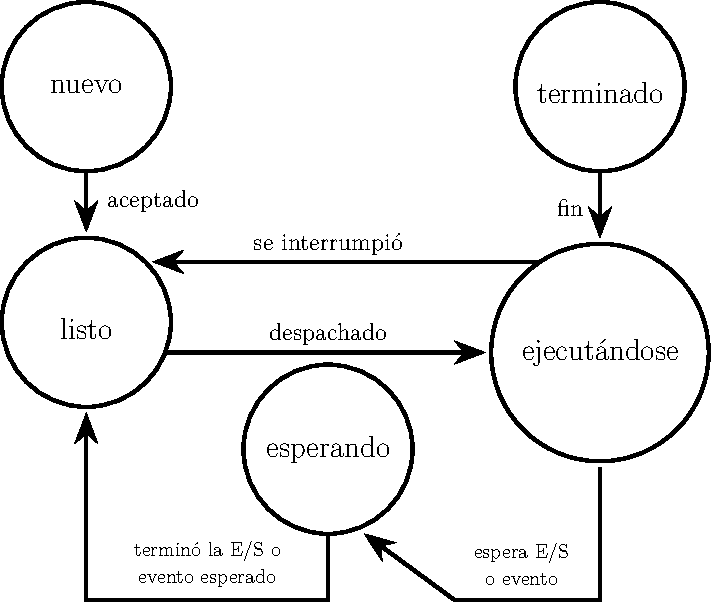
\includegraphics[width=0.5\textwidth]{assets/estados_proceso.pdf}
\end{figure}

\subsection{Process Control Block (PCB)}
Información asociada con cada proceso:
\begin{itemize}
    \item Estado del proceso.
    \item Contador del programa.
    \item Registros del CPU.
    \item Registros del CPU.
    \item Información de calendarización de CPU.
    \item Información de administración de memoria.
    \item Información de contabilización.
    \item Información de estado de I/O.
\end{itemize}

\textbf{Ejemplo de PCB} \par
\begin{tabular}{|p{4cm}|p{4cm}|}
    \hline
    \centering Puntero & \centering Estado del proceso \tabularnewline
    \hline
    \multicolumn{2}{|c|}{Identificador de programa} \\ \hline
    \multicolumn{2}{|c|}{Contador de programa} \\ \hline
    \multicolumn{2}{|c|}{Registros} \\ \hline
    \multicolumn{2}{|c|}{Límites de memoria} \\ \hline
    \multicolumn{2}{|c|}{Información de estado de E/S (Lista de archivos abiertos)} \\ \hline
\end{tabular}





\section{Calendarizadores}
\subsection{Colas de calendarización}
\begin{itemize}
    \item New queue (nuevos): Procesos esperando a ser creados.
    \item Job queue (nuevos, listos y esperando): El conjunto de todos los procesos en el sistema.
    \item Ready queue (listos): El conjunto de todos los procesos residentes en memoria principal listos y en espera de ser atendidos por el CPU.
    \item Device queues (esperando): El conjunto de procesos esperando ser atendidos por un dispositivo de I/O.
\end{itemize}



\subsection{Plazos de calendarización}
\subsubsection{De largo plazo (calendarizador de jobs)}
Selecciona los procesos que serán creados y movidos de la cola de nuevos a la cola de listos (ready).
\begin{itemize}
    \item Es llamado muy infrecuentemente (segundos, minutos) (puede ser más lento).
    \item Controla el grado de multiprogramación
\end{itemize}

\subsubsection{De corto plazo (calendarizador de CPU)}
Selecciona cuál proceso será ejecutado y le asigna el CPU. Además, lo mueve del estado de listos al estado ejecutándose.
\begin{itemize}
    \item Es invocado muy frecuentemente (milisegundos, nanosegundos) debe ser muy rápido.
\end{itemize}
Las decisiones de calendarización de CPU se pueden dar cuando un prodceo:
\begin{itemize}
    \item Cambia de ejecutando (running) al estado esperando (waiting).
    \item Cambia de ejecutando (running) a listo (ready).
    \item Cambia de esperando (waiting) a listo (ready).
    \item Cambia de nuevo a listo (ready).
    \item Termina.
\end{itemize}

Si la calendarización se da exclusivamente bajo las circunstancias 1 y 5 es \textbf{nonpreemptive} (no apropiado). De lo contrario es \textbf{preemptive} (apropiado).

\subsubsection{De mediano plazo}
Selecciona los procesos cuyas páginas de memoria serán intercambiadas a región de swap.



\subsection{Tipos de operaciones}
\begin{itemize}
    \item Orientado a E/S (I/O-Bound): Pasan más tiempo haciendo I/O que procesamiento, tienen periodos (bursts) de CPU muy cortos.
    \item Orientado a CPU (CPU-Bound): Pasan más tiempo haciendo procesamiento; tienen largos periodos de CPU.
\end{itemize}

\subsubsection{Periodos alternos de CPU e I/O}
\begin{tabular}{|*{5}{>{\centering\arraybackslash}m{3cm}|}}
    \hline
    CPU & I/O & CPU & I/O & CPU \\
    \hline
    \makecell{Suma \\ Compara \\ Guarda en archivo}
    & Espera I/O
    & \makecell{Resta \\ Lee de archivo}
    & Espera I/O
    & \makecell{Compara \\ Convierte \\ Guarda en archivo} \\
    \hline
\end{tabular}

\subsection{Despachador}
El despachador cede el control del CPU al proceso seleccionado por el calendarizador a corto plazo. Lo cual implica las siguientes acciones:
\begin{itemize}
    \item Cambio de contexto.
    \item Cambia a modo usuario
    \item Salta a la dirección correcta del proceso del usuario para que reanude su ejecución.
\end{itemize}

\textsl{\textbf{Dispatch latency}}: Tiempo que le toma al despachador parar un proceso y reanudar la ejecución de otro.

\subsection{Criterios de calendarización}
\begin{itemize}
    \item Utilización de CPU: Mantener el CPU tan ocupado como se pueda.
    \item Throughput (rendimiento): Cantidad de procesos que completan su ejecución por unidad de tiempo.
    \item Turnaround time (tiempo de retorno): Cantidad de tiempo que toma la ejecución de un proceso (desde que inicia hasta que termina).
    \item Waiting time (Tiempo de espera): cantidad de tiempo que pasa un proceso esperando en la cola de ready (listos).
    \item Response time (tiempo de respuesta): cantidad de tiempo que toma desde que se envía una solicitud a un proceso hasta que se produce la primera respuesta.
\end{itemize}



\subsection {Criterios de optimización}
\begin{itemize}
    \item Maximizar utilización de CPU.
    \item Maximizar throughput.
    \item Minimizar tiempo de retorno (turnaround time).
    \item Minimizar el tiempo de espear (waiting time).
    \item Minimizar tiempo de respuesta (response time).
\end{itemize}



\subsection{First Come Frist Served}
\textbf{Ejemplo 1} \\
Suponga los siguientes procesos:
\begin{itemize}
    \item P1 cpu burst (24)
    \item P2 cpu burst (3)
    \item P3 cpu burst (3)
\end{itemize}
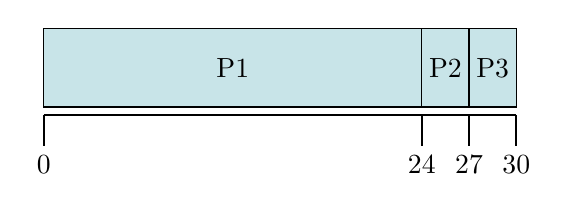
\begin{tikzpicture}[x=0.2cm, y=1cm]
  % Color de los bloques
  \definecolor{ganttblue}{RGB}{200, 228, 232}

  % Bloques de procesos
  \draw[fill=ganttblue, draw=black] (0,0)  rectangle (24,1) node[midway] {P1};
  \draw[fill=ganttblue, draw=black] (24,0) rectangle (27,1) node[midway] {P2};
  \draw[fill=ganttblue, draw=black] (27,0) rectangle (30,1) node[midway] {P3};

  % Eje de tiempo
  \draw[thick] (0,-0.1) -- (30,-0.1);

  % Marcas y etiquetas
  \foreach \x in {0,24,27,30} {
    \draw[thick] (\x,-0.1) -- (\x,-0.5);
    \node[below] at (\x,-0.5) {\x};
  }
\end{tikzpicture} \\
Promedio de tiempos de espera: $(0 + 24 + 27) / 3 = 17$ \\

\textbf{Ejemplo 2} \\
Suponga que los procesos llegan en el orden P2, P3, P1 \\
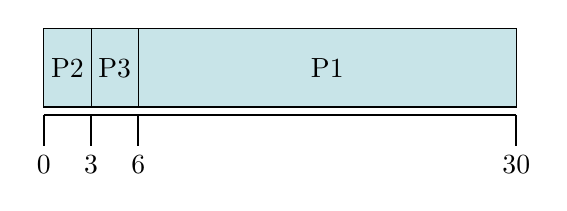
\begin{tikzpicture}[x=0.2cm, y=1cm]
  % Color de los bloques
  \definecolor{ganttblue}{RGB}{200, 228, 232}

  % Bloques de procesos
  \draw[fill=ganttblue, draw=black] (0,0)  rectangle (3,1) node[midway] {P2};
  \draw[fill=ganttblue, draw=black] (3,0) rectangle (6,1) node[midway] {P3};
  \draw[fill=ganttblue, draw=black] (6,0) rectangle (30,1) node[midway] {P1};

  % Eje de tiempo
  \draw[thick] (0,-0.1) -- (30,-0.1);

  % Marcas y etiquetas
  \foreach \x in {0,3,6,30} {
    \draw[thick] (\x,-0.1) -- (\x,-0.5);
    \node[below] at (\x,-0.5) {\x};
  }
\end{tikzpicture} \\
Promedio de tiempos de espera: $(0 + 3 + 6) / 3 = 3$



\subsection{Shortest Job First}
\begin{itemize}
    \item Se asocia con cada proceso la longitud de su siguiente período de CPU.
    \item Se utilizan dichas longitudes para calendarizar primero a los procesos con los tiempos más cortos.
    \item Es óptimo -- da el mínimo tiempo de epsera promedio.
\end{itemize}

\subsubsection{Las dos estrategias}
\textbf{Non-preemptive}: una vez que el CPU se ha asignado al proceso no se le puede quitar hasta que complete su período de CPU. \\

\textbf{Preemptive}: si a la lista de \textsl{ready} llega un nuevo proceso, cuyo período de CPU es más corto que el período de CPU restante del proceso que se está ejecutando, se le quita el CPU. Esta estrategia se conoce como \textbf{Shortest-Remaining-Time-First} (SRTF). \\

\textbf{Ejemplo de Non-Preemptive SJF} \\
\begin{tabular}{|l|l|l|}
    \hline 
    \textbf{Proceso} & \textbf{Tiempo de llegada} & \textbf{Tiempo de CPU} \\
    \hline
    P1 & 0.0 & 7 \\
    \hline
    P2 & 2.0 & 4 \\
    \hline
    P3 & 4.0 & 1 \\
    \hline
    P4 & 5.0 & 4 \\
    \hline
\end{tabular} \\

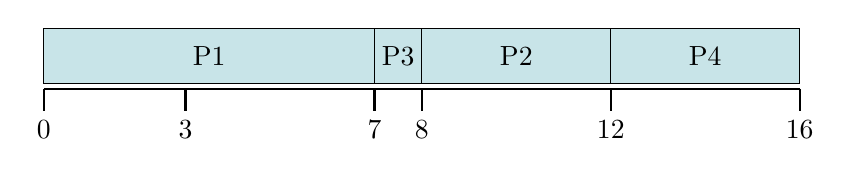
\begin{tikzpicture}[x=0.6cm, y=0.7cm]
  % Color de los bloques
  \definecolor{ganttblue}{RGB}{200, 228, 232}

  % Bloques de procesos
  \draw[fill=ganttblue, draw=black] (0,0) rectangle (7,1) node[midway] {P1};
  \draw[fill=ganttblue, draw=black] (7,0) rectangle (8,1) node[midway] {P3};
  \draw[fill=ganttblue, draw=black] (8,0) rectangle (12,1) node[midway] {P2};
  \draw[fill=ganttblue, draw=black] (12,0) rectangle (16,1) node[midway] {P4};

  % Eje de tiempo
  \draw[thick] (0,-0.1) -- (16,-0.1);

  % Marcas y etiquetas
  \foreach \x in {0,3,7,8,12,16} {
    \draw[thick] (\x,-0.1) -- (\x,-0.5);
    \node[below] at (\x,-0.5) {\x};
  }
\end{tikzpicture} \\

\textbf{Ejemplo de Preemptive SJF} \\
\begin{tabular}{|l|l|l|}
    \hline 
    \textbf{Proceso} & \textbf{Tiempo de llegada} & \textbf{Tiempo de CPU} \\
    \hline
    P1 & 0.0 & 7 \\
    \hline
    P2 & 2.0 & 4 \\
    \hline
    P3 & 4.0 & 1 \\
    \hline
    P4 & 5.0 & 4 \\
    \hline
\end{tabular} \\

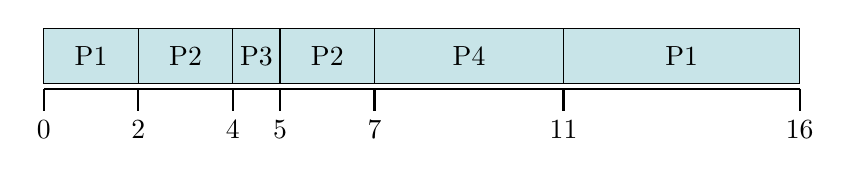
\begin{tikzpicture}[x=0.6cm, y=0.7cm]
    % Color de los bloques
    \definecolor{ganttblue}{RGB}{200, 228, 232}

    % Bloques de procesos
    \draw[fill=ganttblue, draw=black] (0,0) rectangle (2,1) node[midway] {P1};
    \draw[fill=ganttblue, draw=black] (2,0) rectangle (4,1) node[midway] {P2};
    \draw[fill=ganttblue, draw=black] (4,0) rectangle (5,1) node[midway] {P3};
    \draw[fill=ganttblue, draw=black] (5,0) rectangle (7,1) node[midway] {P2};
    \draw[fill=ganttblue, draw=black] (7,0) rectangle (11,1) node[midway] {P4};
    \draw[fill=ganttblue, draw=black] (11,0) rectangle (16,1) node[midway] {P1};

    % Eje de tiempo
    \draw[thick] (0,-0.1) -- (16,-0.1);

    % Marcas y etiquetas
    \foreach \x in {0,2,4,5,7,11,16} 
    {
        \draw[thick] (\x,-0.1) -- (\x,-0.5);
        \node[below] at (\x,-0.5) {\x};
    }
\end{tikzpicture} \\

\subsection{Determinar la longitud del siguiente período de CPU}
\begin{itemize}
    \item Sólo se puede estimar.
    \item Se puede estimar a partir de las longitudes de los períodos de CPU previos, mediante promedios exponenciales.
    \item $t$ = longitud del n-ésimo período de CPU.
    \item $\tau_{n + 1}$ = predicción para el siguiente período de CPU.
    \item $\alpha$, $0 \leq \alpha \leq 1$.
    \item Sea: $\tau_{n + 1} = \alpha t_n + (1 - \alpha)\tau_n$
\end{itemize}


\subsection{Calendarización por prioridades}
\begin{itemize}
    \item Un número (entero) de prioridad es asociado a cada proceso.
    \item El CPU es asignado al proceso con la mayor prioridad (entero más pequeño = más alta prioridad).
    \begin{itemize}
        \item Preemptive
        \item Non-preemptive
    \end{itemize}
    \item SJF es un ejemplo de calendarización por prioridades donde la prioridad esobtenida a partir de las predicciones de las longitudes de los períodos de CPU.
    \item Problema: Starvation (inanición) -- los procesos con bajas prioridades quizá nunca se ejecutarán.
    \item Solución: Aging (envejecimiento) -- conforme el tiempo pasa se le incrementa la prioridad a los procesos.
\end{itemize}


\end{document}
